\documentclass[a4paper,11pt]{report}
%
%--------------------   start of the 'preamble'
%
\usepackage{graphicx,amssymb,amstext,amsmath}
\usepackage{enumerate}
\usepackage{hyperref}
\usepackage[spanish]{babel}
\usepackage[utf8]{inputenc}
\hypersetup{
    colorlinks,
    citecolor=black,
    filecolor=black,
    linkcolor=black,
    urlcolor=black
}
%
%%    homebrew commands -- to save typing
\newcommand\etc{\textsl{etc}}
\newcommand\eg{\textsl{eg.}\ }
\newcommand\etal{\textsl{et al.}}
\newcommand\Quote[1]{\lq\textsl{#1}\rq}
\newcommand\fr[2]{{\textstyle\frac{#1}{#2}}}
\newcommand\miktex{\textsl{MikTeX}}
\newcommand\comp{\textsl{The Companion}}
\newcommand\nss{\textsl{Not so Short}}
%
%---------------------   end of the 'preamble'
%
\begin{document}
%-----------------------------------------------------------
\title{Patrones de Diseño}
\author{Patricio Pérez\\
        Sebastián Rocha\\
        Natalia Tarifeño}
\maketitle

%-----------------------------------------------------------
\title {\textbf{PATRONES DE DISEÑO}}\\

A diario se nos presentan diversos problemas  que debemos enfrentar
y/o solucionar,
muchos de estos problemas tienen características muy similares entre sí, a las cuales ya se les han presentado una solución.\\
Estas soluciones ya desarrolladas y probadas exitosamente son los patrones de diseños,  las
cuales buscan de una manera simple, consistente, efectiva y correcta darnos esta respuesta, evitando errores comunes ya abordados.\\
Una de sus características principales es el ahorro de tiempo al momento de abordar un problema que ya tiene solución.\\
Actualmente existen una gran variedad de patrones de diseños, dentro
de los cuales destacan: singleton, proxy, facade o Modelo Vista Controlador (MVC), Modelo
Vista Template (MVT) , entre otros.\\
En particular nos centraremos en el patrón Modelo Vista Controlador comúnmente llamado MVC por sus siglas.\\

\title { \textbf{MODELO VISTA CONTROLADOR (MVC)}}\\

El modelo vista controlador, separa la lógica de negocios con la interfaz de usuario. Aquí se distinguen 3 capas:

\begin{itemize}
    \item{Modelo}
    \item{Vista}
    \item{Controlador}
\end{itemize}

\begin{figure}[!ht]
\begin{center}
  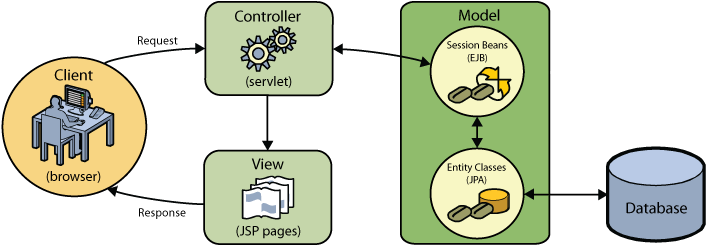
\includegraphics[width=0.9\textwidth]{mvc-diagram.png}
  \caption{MVC aplicado en un software}
\end{center}
\end{figure}


 \newpage
La capa de modelo mapea los datos de la aplicación; en está es en la que almacenaremos datos para buscar/inserción/eliminación y/o modificación.
La capa del controlador es muy importante para este patrón de diseño, ya que es la
que maneja la lógica con la que se manipulan los datos (Es decir se relaciona íntimamente con
la capa modelo) y a su vez interactúa con la capa vista, mostrando al cliente la representación de los datos según sus peticiones.\\

\title {\textbf{ EJEMPLO DE MVC}}\\

\underline{Problema:} Realizar la venta de un producto en una tienda.

\underline{Aplicación del patrón MVC al problema de la tienda:}

En este problema podemos mapear las 3 capas de MVC a la tienda, teniendo lo siguiente:

\begin{itemize}
    \item{Modelo:} Libro de ventas, productos de la tienda, etc. 
    \item{Vista:} Estantes con productos, precio de los productos.
    \item{Controlador:} Vendedor realizando ventas, vendedor realizando boletas.
\end{itemize}

El cliente solicitará al vendedor que le venda un producto (Una frucola grande),
a lo que el vendedor le dirá que esta tiene un precio de \$350 y le pedirá el dinero especificado al cliente.\\
El cliente pagará su producto y el vendedor se lo entregará al cliente con su boleta correspondiente.\\
Cada petición que hace el cliente al vendedor es una interacción con
un controlador, esté a su vez entrega información sobre productos y solicita información al cliente mediante vistas.\\
Se producirán cambios al modelo (ej: Cuando el vendedor le entrega
un producto o la boleta al cliente) y estos son un efecto colateral a las peticiones realizadas al controlador.

\end{document}
